\documentclass{amsart}
\usepackage{amsaddr}
\usepackage{amsmath}
\usepackage{amssymb}
\usepackage{geometry} % see geometry.pdf on how to lay out the page. There's lots.
\geometry{a4paper} % or letter or a5paper or ... etc
\usepackage[utf8]{inputenc}
\usepackage{url}
\usepackage{graphicx}
\usepackage{algorithm}
\usepackage{algorithmic}
\renewcommand{\algorithmicrequire}{\textbf{Input:}}
\renewcommand{\algorithmicensure}{\textbf{Output:}}

\newcommand{\pyumbral}{\textsf{pyUmbral}}
\newcommand{\secp}{\textsf{secp256k1}}

\newcommand{\rk}[2]{rk_{#1\rightarrow#2}}
\providecommand{\pk}[1]{pk_{#1}}
\providecommand{\sk}[1]{sk_{#1}}
\newcommand{\etal}{\emph{et al.\ }}



\title{Umbral: a threshold proxy re-encryption scheme}
\author{David Nuñez}
\address{NICS Lab, University of Malaga, Spain\\\&\\NuCypher Inc. }
\email{dnunez@lcc.uma.es}  
\date{} % delete this line to display the current date

%%% BEGIN DOCUMENT



\begin{document}

\maketitle

\begin{abstract}
This document describes the Umbral proxy re-encryption scheme, as used by NuCypher KMS \cite{egorov2017nucypherkms}. 
Umbral is a threshold proxy re-encryption scheme following a Key Encapsulation Mechanism (KEM) approach. It is inspired by ECIES-KEM \cite{ansi-x9.63}, and the BBS98 proxy re-encryption scheme \cite{blaze1998divertible}. 
With Umbral, Alice (which in the generic name for data owners in NuCypher KMS) can delegate decryption rights to Bob for any ciphertext intended to her, through a re-encryption process performed by a set of $N$ semi-trusted proxies. When at least $t$ of these proxies (out of $N$) participate by performing re-encryption, Bob is able to combine these independent re-encryptions and decrypt the original message using his private key. 
The name ``Umbral'' comes from the Spanish word for ``threshold'', emphasizing this characteristic of the scheme, given its central role in the decentralized architecture of NuCypher KMS. 
\end{abstract}

%\tableofcontents


\section{Introduction}

NuCypher KMS \cite{egorov2017nucypherkms} is a decentralized key management system (KMS), encryption, and access control service. 
It uses proxy re-encryption to delegate decryption rights, enabling this way the private sharing of data between arbitrary numbers of participants in public consensus networks, without revealing data keys to intermediary entities. 

Umbral is a threshold proxy re-encryption scheme loosely inspired by ECIES-KEM \cite{ansi-x9.63} (since the Umbral KEM is constructed similarly as in ECIES) and the BBS98 proxy re-encryption scheme \cite{blaze1998divertible}, although with several improvements to make it non-interactive, unidirectional, and most importantly, verifiable with respect to re-encryption. Finally, the threshold functionality of Umbral reuses ideas from Shamir's Secret Sharing \cite{shamir1979share}, although applied to the context of proxy re-encryption. 

We provide a reference implementation in \cite{pyumbral}, instantiated over an elliptic curve group.

%With respect to the former, Umbral ciphertexts have ``almost'' the same form than ECIES ciphertexts: in both cases, they are composed of an encoded EC point used as ephemeral public key, an encrypted payload using a symmetric encryption algorithm and a MAC code. We say ``almost'' because we introduce some differences that are not supported by the various ECIES specifications; in any case, compliance with ECIES specifications is not one of our goals. 
%
%
%We also remark that we don't use directly Umbral as is, since it is an interactive scheme (i.e., re-encryption key generation requires the secret keys of both Alice and Bob). 
%Instead, we use a generic method to transform any interactive PRE scheme into non-interactive. 

\section{Preliminaries}

\subsection{Notation}

Although the additive notation is the norm when dealing with elliptic curve cryptography, in this document we adopt the multiplicative notation to express the operations in the elliptic curve group, which is the usual approach in the proxy re-encryption literature (where schemes are usually defined in generic groups).

\subsection{A brief introduction to Proxy Re-Encryption}

%(TODO: General description of proxy re-encryption, properties, etc)

Proxy re-encryption is a special type of public-key encryption that permits a proxy to transform ciphertexts from one public key to another, without the proxy being able to learn any information about the original message; to do so, the proxy must be in possession of a \emph{re-encryption key} that enables this process \cite{nunez2017proxy}. Thus, it serves as a means for delegating decryption rights, opening up many possible applications that require of delegated access to encrypted data. In the PRE literature, the parties involved are usually labeled in terms of a relationship of delegation, namely: %. A typical proxy re-encryption environment involves at least three parties:
\begin{itemize}
\item Delegator: This actor is the one that \emph{delegates} his decryption rights using proxy re-encryption. In order to do this he creates a re-encryption key, which he sends to the proxy. We usually refer to the delegator as ``Alice''.
\item Delegatee: The delegatee is granted a delegated right to decrypt ciphertexts that, although were not intended for him in the first place, where re-encrypted for him with permission from the original recipient (i.e., the delegator). This actor usually takes the name ``Bob''.
\item Proxy: It handles the re-encryption process that transforms ciphertexts under the delegator's public key into ciphertexts that the delegatee can decrypt using his private key. The proxy uses the re-encryption key during this process, and does not learn any additional information. 
\end{itemize}

\begin{figure}%[h]
\centering
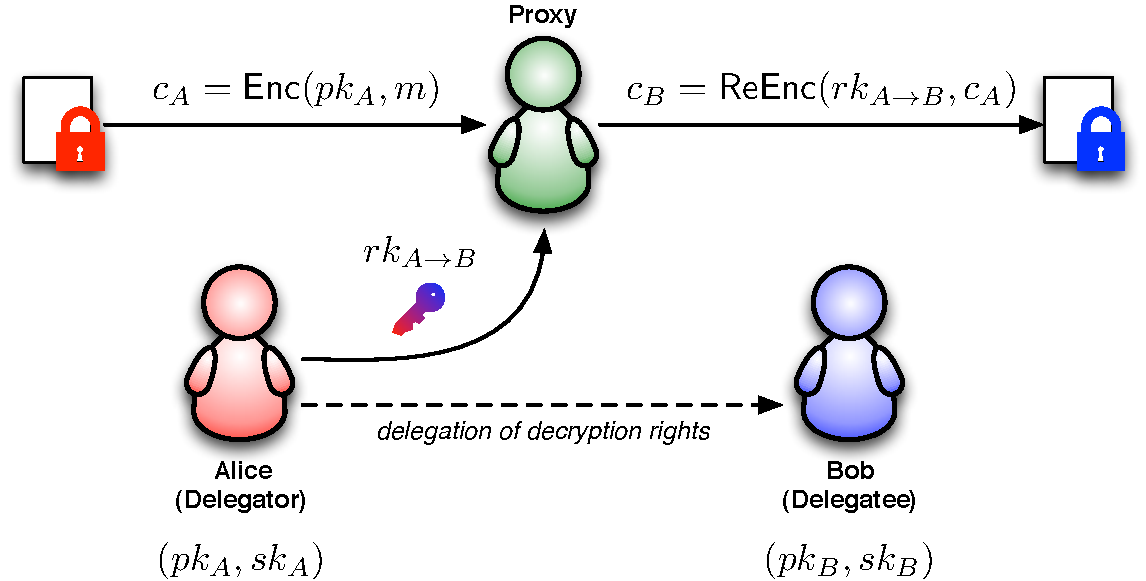
\includegraphics[width=0.75\textwidth]{figures/pre.pdf}
\caption{Main actors and interactions in a PRE environment}
\label{fig:pre-actores}
\end{figure}

Figure~\ref{fig:pre-actores} depicts the main actors in a PRE environment and their interactions. Since PRE is a special type of PKE, users also have a pair of public and private keys, as shown in the figure. Hence, anyone that knows a public key is capable of producing ciphertexts intended for the corresponding recipient; conversely, these ciphertexts can only be decrypted using the corresponding decryption key. 
The distinctive aspect is that ciphertexts can be re-encrypted in order to be decrypted by a different private key than the one originally intended. 



%\subsection{ECIES}
%
%The Asymmetric Encryption Scheme defined in standard ANSI X9.63 \cite{ansi-x9.63}, also known as Elliptic Curve Integrated Encryption Scheme (ECIES), is a hybrid encryption algorithm based on elliptic curve cryptography, symmetric encryption and message authentication codes. 
%This algorithm is of public knowledge, and variants have been standardized also by ISO/IEC 18033-2 \cite{iso-18033-2} and IEEE P1363A \cite{ieee-p1363a}. A comparison of the different variants of ECIES can be found in \cite{gayoso2015security}. 
%
%When producing a ciphertext with ECIES, the sender first creates an ephemeral public key and uses it for a Diffie-Hellman key agreement together with the public key of the intended recipient. The resulting shared secret is used to create the keys for the symmetric encryption and message authentication code algorithms used internally. The final ciphertext consists of the ephemeral public key, as it is necessary for decryption, and the output of the symmetric encryption and message authentication code.
%
%A Sender can  be any entity that generates data and wants to send it confidentially to a receiver, in the form of a ciphertext encrypted under the public key of the receiver. 
%%
%A Receiver can be any entity that is entitled to read ciphertexts encrypted under his public key. We distinguish two types of receivers. The original receiver, which is the recipient of the data originally intended by the sender, and the delegated receiver, whom the original receiver entrusts to be able to decrypt ciphertexts initially intended to him. Therefore, there is a relation of delegation between the original receiver and the delegated one. 
%% 
%The Intermediary is an entity that controls the process of switching the public key of ciphertexts, from the public key of the original receiver to the public key of a delegated receiver, without being able to learn anything from the data. The Intermediary needs a key-switching key between the original and delegated receivers in order to be able to perform the key-switching process.
%
%%ECIES can be used in a variety of elliptic curves, but we will restrict the choice of elliptic curves in our cryptosystem to those that generate a group of prime order. %ECIES define procedures for encryption and decryption, as well as defines 
%
%\subsubsection{Differences between Umbral and ECIES}
%
%The two most important differences we introduce are the following:
%
%\begin{itemize}
%
%\item Single Hash Mode activated: 
%During encryption and decryption, the ephemeral public key is not included in the KDF input. This has some theoretical implications with respect to security, as it can make ECIES encryption malleable. For example, when the KDF only takes the $x$-coordinate of the input EC point, an attacker may replace the ephemeral public key (which is part of the ciphertext) by its inverse; however, this attack is very limited, to the point that Shoup calls this ``benign malleability'' \cite{shoup}. As countermeasure, some ECIES variants allow to include the ephemeral public key as part of the KDF input. In particular, the ISO/IEC 18033-2 standard specification defines an option called Single Hash Mode, which, when activated, removes the ephemeral public key as input to the KDF. Note that this mode is off by default in the ISO/IEC 18033-2 standard (i.e., the ephemeral public key is included).
%
%We must point out that Umbral takes advantage of this malleability during the re-encryption process, in order to transform ciphertexts from one recipient (Alice) to another (Bob). This is done precisely by altering the ephemeral key in the ciphertext. In order to do so, we require that Single Hash Mode is activated so the alteration of the ephemeral key doesn't affect the key derivation process. 
%
%As a final comment, we remark that a certain degree of malleability is unavoidable in any proxy re-encryption scheme, given that its goal is to \emph{transform} ciphertexts from one recipient to another. See \cite{canetti2007chosen} for a deeper discussion on the dichotomy between malleability and re-encryption.
%
%
%\item Authenticated Encryption: The original design of ECIES, in all its variants, uses a symmetric encryption algorithm and a message authentication code for protecting data's confidentiality, integrity and authenticity. However, for the sake of simplicity, we will use a single authenticated encryption primitive that combines all these functionalities. This same approach is used by others, such as the ECIES implementation in Google Tink \cite{tink}. 
%
%\end{itemize}
%
%
%

\section{The Umbral PRE cryptosystem}

In this section we present the Umbral PRE cryptosystem. However, since Umbral is designed following the KEM/DEM approach, our focus will be in the Umbral KEM, since the DEM part is not affected by the ``re-encryption'' process. Note that when referring to ``re-encryption'' we are actually dealing with the transformation of the KEM ciphertexts (or ``capsules''), so technically, it appears it is more appropriate to call this process ``re-encapsulation''. This would lead to the natural sequence of encapsulation/re-encapsulation/decapsulation, as shown in Figure~\ref{fig:umbral-kem}. When possible we will use the term ``re-encapsulation'', although we will continue to use ``re-encryption'' in some contexts such as ``re-encryption keys'', since in the end Umbral KEM will be used as part of a full-fledged proxy re-encryption scheme. 

In this section we will first describe the syntax of the Umbral KEM; next, we present its construction; and finally, its integration with a DEM (i.e., a symmetric encryption algorithm) to produce the Umbral proxy re-encryption scheme. 

\begin{figure}%[h]
\centering
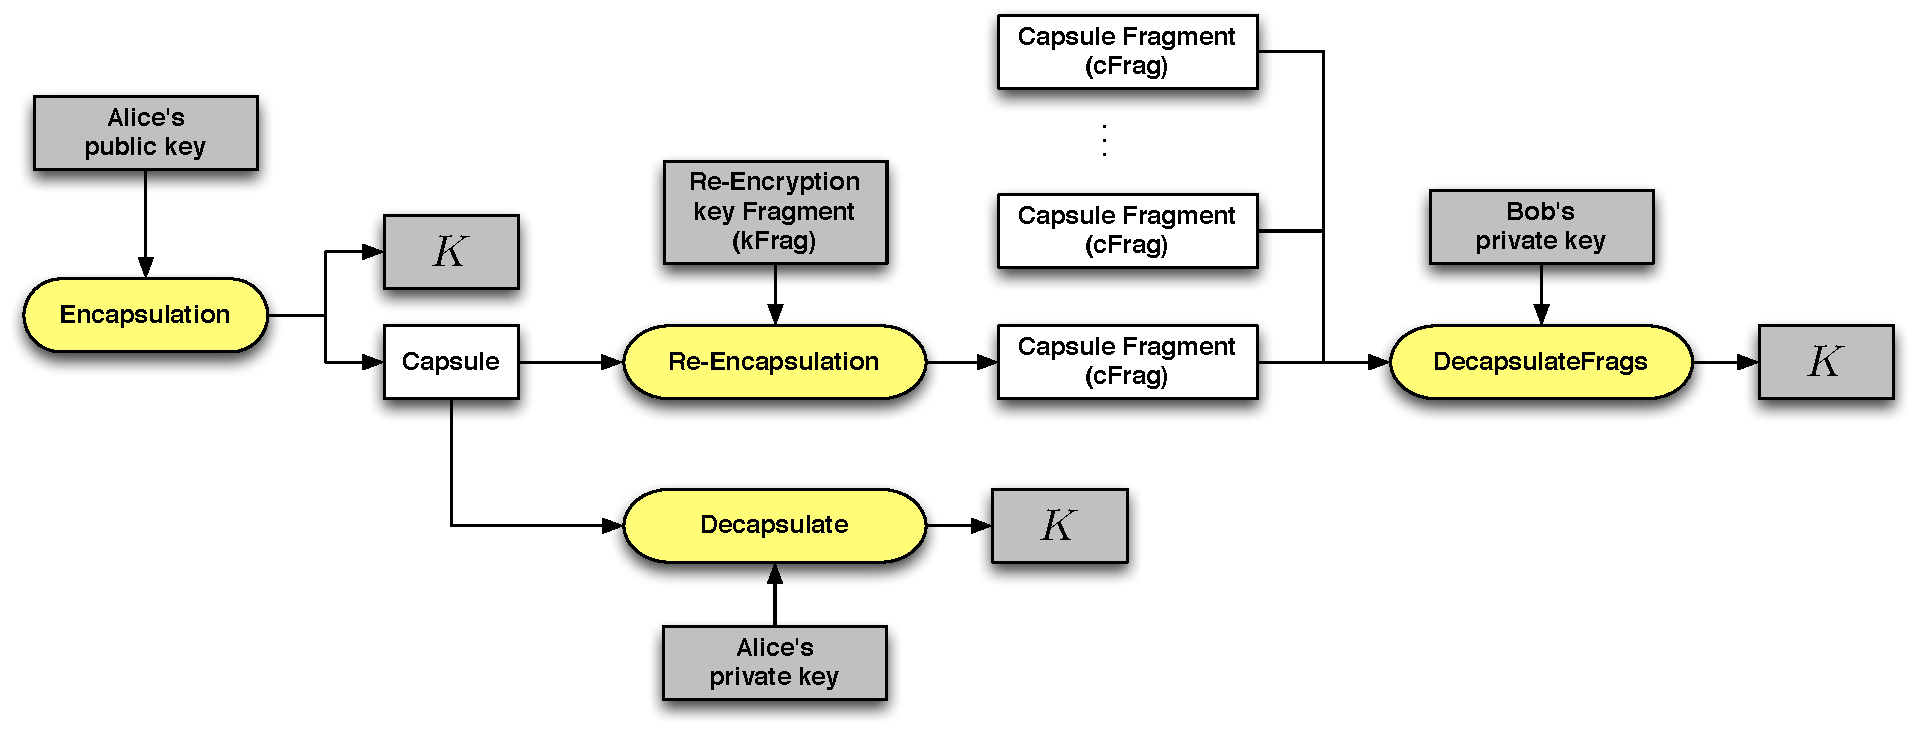
\includegraphics[width=\textwidth]{figures/umbral-kem-flow.pdf}
\caption{Main operation of Umbral KEM. Operations are shown in yellow, cryptographic keys in gray, and data in white}
\label{fig:umbral-kem}
\end{figure}

\subsection{Syntax of the Umbral KEM}

The following is a description of the basic functions provided by Umbral KEM. For clarity we have categorized these functions in different groups according to their functionality. 

\subsubsection{Key Generation Algorithms}

\begin{itemize}

	\item $\mathsf{KeyGen}()$: The key generation algorithm $\mathsf{KeyGen}$ outputs a pair of public and secret keys $(\pk{A}, \sk{A})$.
	\item $\mathsf{ReKeyGen}(sk_A, pk_B, N, t)$: On input the secret key $sk_{A} = a$, the public key of the intended delegatee $pk_{B} = g^b$, a number of fragments $N$, and a threshold $t$, the re-encryption key generation algorithm $\mathsf{ReKeyGen}$ computes $N$ fragments of the re-encryption key between $A$ and $B$, each of them named $kFrag$. 
\end{itemize}


\subsubsection{Encapsulation and Decapsulation}

\begin{itemize}
	\item $\mathsf{Encapsulate}(pk_A)$: On input the public key $pk_A$, the encapsulation algorithm $\mathsf{Encapsulate}$ a symmetric key $K$ and a $capsule$ that allows to derive again (i.e., ``decapsulate'') the symmetric key $K$. 
	
	\item $\mathsf{Decapsulate}(sk_A, capsule)$: On input the secret key $sk_A$, and an original $capsule$, the decapsulation algorithm $\mathsf{Decapsulate}$ outputs the symmetric key $K$, or $\perp$ if the capsule is invalid. 
	
	\item $\mathsf{DecapsulateFrags}(sk_B, \{cFrag_i\}_{i=1}^t)$: On input the secret key $sk_B$, and a set of $t$ capsule fragments or $cFrags$, the algorithm outputs the symmetric key $K$, or $\perp$ if the decryption fails. 
	
\end{itemize}

\subsubsection{Re-Encapsulation}%ryption and Verification of Re-Encryption}

\begin{itemize}
\item $\mathsf{ReEncapsulation}(kFrag, capsule)$: On input a re-encryption key fragment $kFrag$, and a $capsule$, the re-encapsulation algorithm $\mathsf{ReEncapsulation}$ outputs the capsule fragment $cFrag$, or $\perp$ if the the process fails.

\end{itemize}

\subsection{The Umbral KEM construction}

\subsubsection{Setup and public parameters}\label{sec:setup_umbral}

\begin{itemize}

\item $\mathsf{Setup}(sec)$: The setup algorithm first determines a cyclic group $\mathbb G$ of prime order $q$, according to the security parameter $sec$. Let $g, U\in \mathbb G$ be generators. Let $H_2: \mathbb G^2 \to \mathbb Z_q$, $H_3: \mathbb G^3 \to \mathbb Z_q$, and $H_4: \mathbb G^3 \times Z_q \to \mathbb Z_q$ be hash functions that behave as random oracles. Let $\mathsf{KDF}: \mathbb G \to \{0,1\}^\ell$ be a key derivation function also modeled as a random oracle, where $\ell$ is according to the security parameter $sec$. The global public parameters are represented by the tuple:
$$params = (\mathbb G, g, U, H_2, H_3, H_4, \mathsf{KDF})$$

\end{itemize}

For simplicity, we will omit the public parameters from the rest of the functions. 

\subsubsection{Key Generation Algorithms}

\begin{itemize}
	%\item $\mathsf{Setup}(1^k)\rightarrow params$. On input the security parameter $1^k$, the global setup algorithm $\mathsf{Setup}$ outputs the global parameters $params$.
	\item $\mathsf{KeyGen}()$: Sample $a \in \mathbb Z_q$ uniformly at random, compute $g^a$ and output the keypair $(pk, sk) = (g^a, a)$.

	\item $\mathsf{ReKeyGen}(sk_A, pk_B, N, t)$: On input the secret key $sk_{A} = a$, the public key of the intended delegatee $pk_{B} = g^b$, a number of fragments $N$, and a threshold $t$, the re-encryption key generation algorithm $\mathsf{ReKeyGen}$ computes $N$ fragments of the re-encryption key between $A$ and $B$ as follows:
	
	\begin{enumerate}
\item Sample random $x_A \in \mathbb Z_q$ and compute $X_A = g^{x_A}$
\item Compute $ d = H_3(X_A, pk_B, (pk_B)^{x_A})$. Note how $d$ is the result of a non-interactive Diffie-Hellman key exchange between $B$'s keypair and the ephemeral key pair $(x_A, X_A)$. We will use this shared secret to make the re-encryption key generation of the scheme non-interactive.
\item Sample random $t-1$ elements $f_i\in \mathbb Z_q$, with $1 \leq i \leq t-1$, and  compute $f_0 = a \cdot d^{-1} \bmod q$.
\item Construct a polynomial $f(x) \in \mathbb Z_q[x]$ of degree $t-1$, such that $f(x) = f_0 + f_1x + f_2x^2 + ... + f_{t-1}x^{t-1}$.  
\item Compute $ D = H_6(pk_A, pk_B, pk_B^a)$
\item Initialize set $KF = \emptyset$ and repeat $N$ times:

    \begin{enumerate}
    \item Sample random $y, id \in \mathbb Z_q$
    \item Compute $s_x = H_5(id, D)$ and $Y = g^y$.
    \item Compute $rk = f(s_x)$ 
    \item Compute $U_1 = U^{rk}$.
    \item Compute $z_1 = H_4(Y, id, pk_A, pk_B, U_1, X_A)$, and $z_2 = y - a \cdot z_1$.
    \item Define a re-encryption key fragment $kFrag$ as the tuple $(id, rk, X_A, U_1, z_1, z_2)$.
    \item $KF = KF \cup \{kFrag\}$
	\end{enumerate}

\item Finally, output the set of re-encryption key fragments $KF$.
\end{enumerate}
\end{itemize}


\subsubsection{Encapsulation and Decapsulation}

\begin{itemize}
	\item $\mathsf{Encapsulate}(pk_A)$: On input the public key $pk_A$, the encapsulation algorithm $\mathsf{Encapsulate}$ first samples random $r, u \in \mathbb Z_q$ and computes $E = g^r$ and $V = g^u$. 
	Next, it computes the value $s = u + r \cdot H_2(E, V)$. 
	The derived key is computed as $K = \mathsf{KDF}((pk_A)^{r + u})$. 
	The tuple $(E, V, s)$ is called $capsule$ and allows to derive again (i.e., ``decapsulate'') the symmetric key $K$. 
	Finally, the encapsulation algorithm outputs $(K, capsule)$.	
	
	\item $\mathsf{CheckCapsule}(capsule)$: On input a $capsule = (E, V, s)$, this algorithm examines the validity of the capsule by checking if the following equation holds:
	$$ g^s \stackrel{?}{=} V \cdot E^{H_2(E, V)}$$
	
	\item $\mathsf{Decapsulate}(sk_A, capsule)$: On input the secret key $sk_A = a$, and an original $capsule = (E,V,s)$, the decapsulation algorithm $\mathsf{Decapsulate}$ first checks the validity of the capsule with $\mathsf{CheckCapsule}$ and outputs $\perp$ if the check fails. Otherwise, it computes $K = \mathsf{KDF}((E\cdot V)^{a})$. Finally, it outputs $K$.
	
	\item $\mathsf{DecapsulateFrags}(sk_B, pk_A, \{cFrag_i\}_{i=1}^t)$: On input the secret key $sk_B = b$, the original public key $pk_A = g^a$, and a set of $t$ capsule fragments, being each of them $cFrag_i = (E_{1,i}, V_{1,i}, id_i, X_A)$, the fragments decapsulation algorithm $\mathsf{DecapsulateFrag}$ does the following:
	
	\begin{enumerate}
	\item Compute $ D = H_6(pk_A, pk_B, pk_A^b)$
    \item Let $S = \{s_{x,i}\}_{i=1}^t$, for $s_{x,i} = H_5(id_i, D)$. For all $s_{x,i}\in S$, compute:
    \[\lambda_{i, S} = \prod\limits_{j=1, j\neq i}^{t} \frac{s_{x,j}}{s_{x,j}-s_{x,i}}\]
    \item Compute the values:
     	$$E' = \prod\limits_{i=1}^{t} (E_{1,i})^{\lambda_{i, S}}	
		\qquad
		V' = \prod\limits_{i=1}^{t} (V_{1,i})^{\lambda_{i, S}}$$
	\item Compute $d = H_3(X_A, pk_B, X_A^b)$. Recall that $d$ is the result of a non-interactive Diffie-Hellman key exchange between $B$'s keypair and the ephemeral key pair $(x_A, X_A)$. Note also that the value $X_A$ is the same for all the $cFrags$ that are produced by re-encryptions using a $kFrag$ in the set of re-encryption key fragments $KF$. 
	\item Finally, output the symmetric key $K= \mathsf{KDF}((E'\cdot V')^{d})$. 
	\end{enumerate}
\end{itemize}

\subsubsection{Re-Encapsulation}%ryption and Verification of Re-Encryption}

\begin{itemize}
\item $\mathsf{ReEncapsulate}(kFrag, capsule)$: On input a re-encryption key fragment $kFrag= (id, rk, X_A, U_1, z_1, z_2)$, and a $capsule = (E,V,s)$, the re-encapsulation algorithm $\mathsf{ReEncapsulate}$ first checks the validity of the capsule with $\mathsf{CheckCapsule}$ and outputs $\perp$ if the check fails. Otherwise, it computes $E_1 = E^{rk}$ and $V_1 = V^{rk}$, and outputs the capsule fragment $cFrag = (E_1, V_1, id, X_A)$. 




\end{itemize}

		

\subsection{The KEM/DEM construction}

Extending Umbral KEM with a DEM results in a full-fledged proxy re-encryption scheme. As such, this defines encryption and decryption algorithms, rather than encapsulation and decapsulations. We require the DEM to be an authenticated encryption with associated data algorithm, which we will denote as $\mathsf{AEAD}$. Note also how the re-encryption algorithm actually does not involve any symmetric encryption operation. We omit the key generation algorithms since they are not changed in the extension. 

\begin{itemize}
	
	\item $\mathsf{Encrypt}(pk_A, M)$: On input the public key $pk_A$ and a message $M\in\mathcal{M}$, the encryption algorithm $\mathsf{Encrypt}$ first computes $(K, capsule) = \mathsf{Encapsulate}(pk_A)$. 
	$encData$ is the result of applying $\mathsf{AEAD}$ to $M$ with key $K$, with $capsule$ as associated data. 
	Finally, it outputs the ciphertext $C = (capsule, encData)$.
	
	\item $\mathsf{Decrypt}(sk_A, C)$: On input the secret key $sk_A$ and a ciphertext $C = (capsule, encData)$, the decryption algorithm $\mathsf{Decrypt}$ computes the key $K = \mathsf{Decapsulate}(sk_A, capsule)$, and decrypts ciphertext $encData$ using the decryption function of $\mathsf{AEAD}$ with key $K$ and $capsule$ as associated data, which results in message $M$ if decryption is correct, and $\perp$ otherwise. Finally, it outputs message $M$ (or $\perp$ if decryption was invalid).
	
	\item $\mathsf{ReEncrypt}(kFrag, C)$: On input a re-encryption key fragment $kFrag$ and a ciphertext $C = (capsule, encData)$, the re-encryption algorithm $\mathsf{ReEncrypt}$ applies $\mathsf{ReEncapsulate}$ to the $capsule$ to obtain a $cFrag$, and outputs the re-encrypted ciphertext $C' = (cFrag, encData)$.
	
	\item $\mathsf{DecryptFrags}(sk_B, \{C'_i\}_{i=1}^t)$: On input the secret key $sk_B$, a set of $t$ re-encrypted ciphertexts $C'_i = (cFrag_i, encData)$, the fragments decryption algorithm $\mathsf{DecryptFrags}$ first decapsulates the $cFrags$ with $\mathsf{DecapsulateFrags}(sk_B, \{cFrag_i\}_{i=1}^t)$ to produce key $K$, and decrypts ciphertext $encData$ using the decryption function of $\mathsf{AEAD}$ with key $K$ and $capsule$ as associated data, which results in message $M$ if decryption is correct, and $\perp$ otherwise. Finally, it outputs message $M$ (or $\perp$ if decryption was invalid).	Note that the symmetric ciphertext $encData$ is the same for all the $C'_i$ that are re-encryptions of the same ciphertext $C$. 
	
\end{itemize}
	


\section{Notes concerning Umbral reference implementation (\textsf{pyUmbral})}

\subsection{Choice of elliptic curve}
The only restriction that the Umbral cryptosystem imposes on the choice of EC curve is that it should generate a group of prime order, since we need to compute inverses modulo the order of this group. In our current setting, we use the \textsf{secp256k1} curve since it fulfills this latter requirement and it is widely used in the blockchain ecosystem; we are exploring other curve choices that could improve performance. 

\subsection{Hash functions}
As described in Section~\ref{sec:setup_umbral}, Umbral requires several hash functions, namely $H_2: \mathbb G^2 \to \mathbb Z_q$, $H_3: \mathbb G^3 \to \mathbb Z_q$, and $H_4: \mathbb G^3 \times Z_q \to \mathbb Z_q$, which behave as random oracles. Since for elements of both $\mathbb G$ and $\mathbb Z_q$ there exists efficient encodings to bit string (i.e., compressed representation in the case EC points and ), in \textsf{pyUmbral} we implement $H_2, H_3$ and $H_4$ from a common hash function $H': \{0,1\}^* \to \mathbb Z_q$. For example, for the case of $H_2$, we define it as $H_2(g_1, g_2) = H'(\mathsf{encode}(g_1)||\mathsf{encode}(g_2))$.

This reduces the problem to the definition of $H'$. Let $n$ be the order of the group induced by the curve in use, and $d$ the size in bits of an internal hash function (e.g., \textsf{BLAKE2b}). Algorithm~\ref{alg:hash_to_bn} describes how to compute $H'$. 


\begin{algorithm} % enter the algorithm environment
\caption{Pseudocode for $H'$ (\texttt{hash\_to\_bn} in \pyumbral)} % give the algorithm a caption
\label{alg:hash_to_bn} % and a label for \ref{} commands later in the document
\begin{algorithmic} % enter the algorithmic environment
	\REQUIRE $X$ is a bit string of arbitrary size
    \STATE $i \Leftarrow 0$
	\REPEAT
		\STATE $r \Leftarrow \mathsf{int}(\mathsf{digest}(X||\mathsf{encode}(i))) \bmod n$
		\STATE $i \Leftarrow i + 1$
	\UNTIL{$r > 2^d \bmod n$}
	\RETURN $r$
\end{algorithmic}
\end{algorithm}

For reference, in the case of curve \secp~and a 64-bytes digest ($d=512$):
\begin{align*} 
n &= \mathtt{0xfffffffffffffffffffffffffffffffebaaedce6af48a03bbfd25e8cd0364141} \\ 
2^d \bmod n &= \mathtt{0x9d671cd581c69bc5e697f5e45bcd07c6741496c20e7cf878896cf21467d7d140}
\end{align*}

\subsection{Symmetric encryption}
As per the authenticated encryption scheme, we use PyNaCl's SecretBox implementation, which in turn uses Chacha20-Poly1305.

\subsection{Key derivation}
For the KDF, we use \textsf{HKDF} with \textsf{BLAKE2b} as hash function, with a digest size of 64 bytes. 

%\subsection{Nothing-up-my-sleeve generation of public parameters}
%Umbral requires a group element $U$ that is used as another generator. In order to 


\bibliographystyle{unsrt}       % APS-like style for physics
\bibliography{umbral-doc}
\end{document}